\documentclass{beamer}

\mode<presentation>
{
  \usetheme{default}
  \usecolortheme{beaver}
  \setbeamercovered{transparent}
  \setbeamertemplate{caption}[numbered]
}

\usepackage{booktabs}
\usepackage{float}
\usepackage{siunitx}
\usepackage{subfloat}
\usepackage{subfig}
% \usepackage[labelsep=none,labelformat=empty]{caption}
\usepackage{caption}

\renewcommand{\tablename}{}
\newcommand{\ra}[1]{\renewcommand{\arraystretch}{#1}}

\title
{
    Gait Event Detection Using an LSTM Network
}

\subtitle
{
    10-701
    % Introduction to Machine Learning
    Project Presentation
}

\author
{
    Pablo Iturralde\\
    Yin Zhong\\
    Jakob Bauer
    % Pablo A. Iturralde,
    % Yin Zhong,
    % Jakob Bauer
}

\date
{
    April 22, 2015
}

% ==============================================================================

\begin{document}

\begin{frame}
  \titlepage
\end{frame}

\begin{frame}{Introduction}
    \begin{itemize}
        \item
            Goal: detect gait events (heel strike, toe off) 
            in motion capture data
        \item
            Necessary to measure changes in gait that arise from training,
            disease or aging
    \end{itemize}
    \begin{figure}
    \begin{center}
        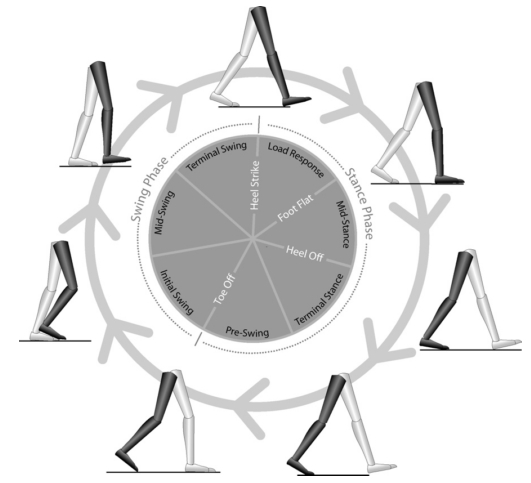
\includegraphics[width=0.5\textwidth]{figures/gait_events.jpg}
        \caption{Gait events [Rueterbories et al., 2010]}
    % \label{fig:barplot}
    \end{center}
    \end{figure}
\end{frame}

\begin{frame}{Data}
    \begin{itemize}
        \item
            Time series data
        \item
            54 features 
            (18 motion capture markers $\times$ 3 dimensions)
        \item
            \num{240000} samples 
            (8 subjects $\times$ 3 trials $\times$ \num{10000} samples)
        \item
            Groundtruth from force plates
    \end{itemize}
\end{frame}

\begin{frame}{Baseline Methods}
    \begin{itemize}
        \item
            Signal processing approach [O'Connor et al., 2007]
            \begin{itemize}
                \item
                    Heuristic based on speed of heel and toe markers
                \item
                    No learning
                \item
                    Sensitive to threshold value
            \end{itemize}
        \item
            Feed-forward Neural Network [Miller, 2009]
            \begin{itemize}
                \item
                    Sliding window centered around the desired marker
                \item
                    Requires heavy preprocessing (dimensionality reduction,
                    variable window size based on foot speed)
            \end{itemize}
    \end{itemize}
\end{frame}

\begin{frame}{Our Approach: LSTM}
    \begin{itemize}
        \item
            LSTM = Recurrent Neural Network with memory cells
        \item
            Motivation
            \begin{itemize}
            \item
                Detect long-range dependencies
            \item
                No windowing required
            \end{itemize}
        \item
            Network architecture
            \begin{itemize}
                \item TODO
            \end{itemize}
        \item
            Implementation
            \begin{itemize}
                \item
                    Torch/Lua
                \item
                    LSTM cell by
                    de Freitas (Oxford University, Google Deepmind)
                \item
                    AWS EC2 GPU instance (g2.2xlarge)
            \end{itemize}
    \end{itemize}
\end{frame}

\begin{frame}{Results}
\end{frame}

\begin{frame}{Q\&A}
    \Large
    \centering
    Thank you for your attention!
\end{frame}

\end{document}
